\documentclass[letterpaper,twocolumn,openany,nodeprecatedcode]{dndbook}


\usepackage[italian]{babel}

\usepackage[utf8]{inputenc}
\usepackage{lipsum}
\usepackage{listings}
\usepackage{shortvrb}
\usepackage{stfloats}
\usepackage{datetime2}
\usepackage{graphicx}
\graphicspath{ {figures/} }
\usepackage{array}
\usepackage{titling}

\usepackage{tabularx}
\usepackage{blindtext,booktabs}
\usepackage{caption} % for '\caption*' macro

\pretitle{\begin{center}\fontsize{18bp}{18bp}\selectfont}
   \posttitle{\vspace{14bp}\par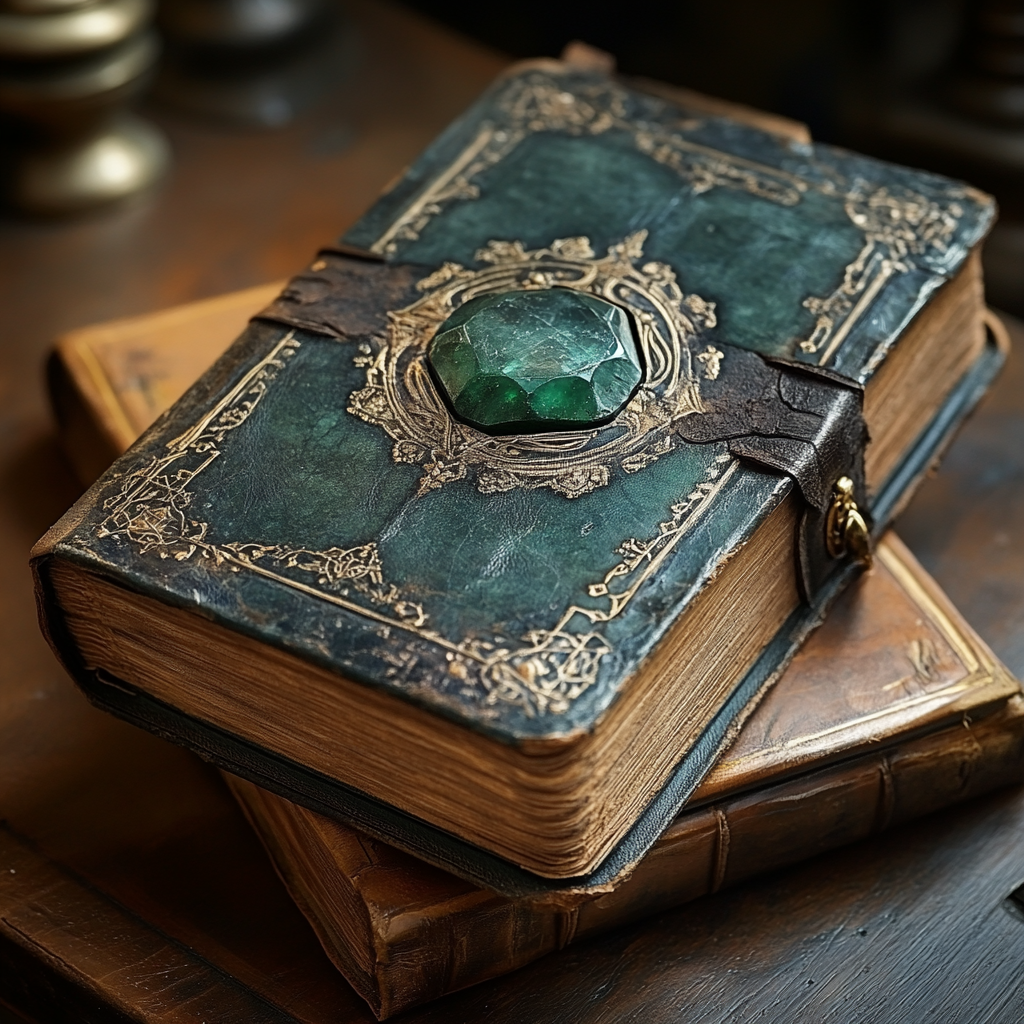
\includegraphics[width=170mm]{logo}\par\end{center}}
\preauthor{\begin{center}\fontsize{14bp}{14bp}\selectfont}
   \postauthor{\par\end{center}}
\predate{\begin{center}}
   \postdate{\par\end{center} }

\title{ }

\title{%
  Addon per D\&D: \\
  \large Il grimorio del Mago Selvaggio}
\author{Matteo Scarpa - Fundor333}
\date{\today}


\newcommand{\nomecampagna}{\textit{Kebab e patatine fritte}} %\textit{Alberi del sigillo}}
\newcommand{\mottocampagna}{\textit{Magari anche delle cipolle fritte}}


\begin{document}

\maketitle

\tableofcontents

\mainmatter

\chapter{Introduzione}

\DndDropCapLine{Q}uesto é un piccolo pdf dove vengono inserite tutte le aggiunte che ho creato o raccolto da amici e giocatori per conservarli e averli pronti ad uso. A meno che non sia specificato espressamente, tutto il materiale è stato creato per la 5a edizione di D\&D.


\chapter{Classi}
\DndDropCapLine{N}on essendo soddisfatto di alcune cose delle classi ho aggiunto e/o fatto modifiche in modo che torni comodo per le mie campagne.
Quanto scritto qui è stato bilanciato per la campagna che ho in mente, ma non è detto che sia bilanciato per altre campagne.

Inoltre, alcune classi sono state modificate per essere più simili a quelle di D\&D 3.5, ma non tutte.
Se avete delle idee per migliorare le classi, o se avete trovato degli errori, potete contattarmi su Discord o su GitHub.


\section{Warlock}

\subsection{Patto dell'intrattenitore}
Il patrono dona al Warlock uno strumento per intrattenere che, se perde o viene distrutto, può riceverne un altro dopo aver effettuato una cerimonia di 1 ora. Se lo fa quello precedente sparisce in una cacofonia di suoni.
Lo strumento conta come oggetto magico a i fini di abilità e incantesimi e se distrutto in qualunque modo emette una cacofonia (suono 18m). Il warlock può usarlo 2 volte al giorno per dare Ispirazione Bardica (vedi bardo) ma con il dado  subito più piccolo rispetto al bardo.
Questo strumento può essere usato come catalizzatore per il bardo per gli incantesimi fino al 5º livello incluso

\captionof{table}{Patto dell'intrattenimento dadi}
\label{pattointrattenimentodado}
\begin{DndTable}{cX}
\textbf{Livello minimo} & \textbf{Dado} \\
3 & D4 \\
5 & D6 \\
10 & D8 \\
15 & D10 \\
\end{DndTable}



\begin{DndSidebar}[float=!h]{Doni del patto}
Ogni opzionedi Dono del Patto genera una creatura o un oggetto
speciale, che riflette la natura del patrono del warlock.
\subparagraph{Patto della Catena} Il famiglia del warlock è più intelligente dei famigli normali. La sua forma standard può riflettere l'essenza del suo patrono: gli spiri telli e gli pseudodraghi sono collegati al Signore Fatato, mentre gli imp e i quasit sono collegati all'Immondo. Dato che la natura del Grande Antico è imperscrutabile, qualsiasi tipo d i famiglia può essere coll egato a lui. Per quanto riguarda il Ringmaster il famiglio sarà un animale del circo di piccola taglia mentre per il patrono del Ventaglio sarà un piccolo e delicato rapace della famiglia dei gufi e civette
\subparagraph{Patto della Lama} Se il patrono del warlock è il Signore Fatato, la sua arma potrebbe essere un' esile lama avvolta d a foglie e rampicanti. Se il warlock serve l'Immondo, la sua arma potrebbe essere un'ascia fatta di metallo nero e decorata di simboli fiammeggianti. Se il patrono del warlock è il Grande Antico, la sua arma potrebbe essere una lancia dall'aspetto antico, con una gemma incastonata nella punta e intagliata per sembrare un inquietante occhio privo di palpebre. Per quanto riguarda il Ringmaster l'arma potrà essere o una frusta da domatore o un bastone animato (bastone con una lama dentro). In entrambi i casi alla fine dell'impugnatura ci sarà una pietra che viene a ricordare il tendone del circo ma da la sensazione che respiri. Per quanto riguarda invece il patrono del Ventaglio l'arma è una sottilissima spada lunga, con una lama quasi invisibile e con una impugnatura di legno senza guardia. Una piccola foglia di quello che sembra essere cuoio segue come per magia il manico della spada, ma guardando meglio, è legata al manico da quello che sembra essere un capello
\subparagraph{Patto del Tomo} Il Libro delle Ombre del warlock potrebbe essere un raffinato volume dall a copertina rifinita in oro, contenente vari incantesimi di ammaliamento e di illusione, consegnatogli dal nobile Signore Fatato.
Oppure potrebbe essere un ponderoso tomo rilegato i n pelle demoniaca e borchie metalliche, pieno di incantesimi di evocazione e informazioni proibite sulle più sinistre regioni del cosmo, in quanto dono dell'Immondo. Oppure potrebbe invece essere il diari o lacero di un pazzo, precipitato nella follia dopo essere entrato in contatto con ìl Grande Antico: un libro compostoda frammenti di incantesimi che solo il warlock, grazie alla follia che si sta insinuando anche nella sua mente, è in grado di comprendere e lanciare. Un libro di legno ricoperto di stoffa di un tendone da circo e riempito di incantesimi ruomorosi e scenici riempie il tomo del Ringmaster. Una pergamena fissata a due bastoni di ciliegio riccamente decorati ma rovinati dal tempo e sigillati da una foglia di quello che sembra cuoio. All'interno sono contenuti incantesimi che usano il suono e comandano i venti sviluppati dal patrono del Ventaglio
	\subparagraph{Patto dell'intrattenitore}
   Se il patrono del warlock è il Signore Fatato, lo strumento potrebbe essere un violino, una cornamusa sarebbe più facilmente collegata all'Immondo.
   Ovviamente il Grande Antico e gli Esterni non hanno uno strumento specifico.
   Invece per quanto riguarda Ringmaster è una elegante frusta mentre per il patrono del Ventaglio è una coppia di ventagli collegati con una catena di pietre colorate.
\end{DndSidebar}

\subsection{Patrono Ringmaster}
Il patrono del Warlock fa parte di un circo o una arena di dubbia origine, di sicuro non è una arena o un circo 'normale'. Solitamente si occupano di raccogliere emozioni con i loro spettacoli partecipando loro stessi o mandando avanti i loro intrattenitori. Nonostante il nome lo faccia pensare possono non essere il Ringmaster del circo ma può essere il bigliettaio con l'occhio veloce o la sfinge che fa lo spettacolo con gli acrobati. Una cosa però è sicura: non si rivela a chi non fa parte del loro circolo ristretto ed è possibile che un suo warlock sappia solo il nome del patrono e a che circo/arena sono collegati.
Solitamente il warlock viene preso per raccogliere emozioni per continuare l'attività di "famiglia".

\subsection{Patrono del Ventaglio}

Il patrono del warlock è una leggenda, ancora più antica del Signore Fatato, che ha perso talmente potere che ha perso struttura fisica e rimane come una versione quasi non morta di se stesso/a. Vista la condizione e che ha spesso origini fatate, il patrono controlla illusioni e suoni e non si sposta dalla sua "base" ma è solitamente facilmente riconoscibile in quanto si nasconde dietro un ventaglio e veli per alterare la percezione di se.
Il patrono del Ventaglio solitamente è un santone in cima a una montagna o la signora a capo del palazzo del piacere locale o sigillato in qualche posto ma comunque obbligato da forze maggiori a non poter lasciare il posto. Solitamente il warlock viene usato dal patrono come proprio agente per far recuperare al patrono la possibilità di muoversi da dove è "relegato"


\chapter{Tabelle}
\DndDropCapLine{Q}uesta sezione contiene le nuove tabelle che io e i miei compagni di avventura abbiamo accumulato nel tempo. 


\section{The Hangover - Una notte da leoni}
\label{sec:hangover}
Questo è un piccolo tavolo per generare oggetti casuali che i personaggi potrebbero trovare al risveglio dopo una notte di bagordi. Può essere usato per aggiungere un tocco di umorismo o sorpresa alla sessione di gioco.

\begin{DndTable}[color=PhbLightCyan]{cX}
\textbf{d8} & \textbf{Item} \\
1 & Sposa lo gnomo addetto alle richieste della gilda \\
2 & Sposa un altro PG \\
3 & Ha vinto 1000 mo \\
4 & Deve delle monete (1000 mo) a uno strozzino (1D2 per vedere se mafioso o strozzino)\\
5 & Si risveglia nella fontana della cittá (1D2 per vedere se vestito)\\
6 & Si sveglia nella taverna (1D2 per vedere se vestito)\\
7 & Si risveglia nudo in un letto con un altro PG \\
8 & Si sveglia con 1D6 prostitute (1D2 per scegliere il sesso) \\
9 & Si risveglia con un tatuaggio di un drago sulla schiena \\
10 & Ha una coppa magica nello zaino \\
11 & Ha un anello magico che non riesce a togliere \\
12 & É perseguitato da fuochi fatui che lo seguono ovunque \\
\end{DndTable}



\chapter{Appendici}
\end{document}


